%! TEX program = lualatex
\documentclass[a4paper, 12pt]{article}

\usepackage[margin=2.5cm]{geometry}
\usepackage{microtype}
\usepackage{indentfirst}
\usepackage{polyglossia}
\usepackage[colorlinks=true, allcolors=black]{hyperref}
\usepackage{graphicx}
\usepackage[font=footnotesize, labelfont=bf]{caption}
\usepackage{wrapfig}
\usepackage{amsmath}
\usepackage{mathrsfs}
\usepackage{icomma}
\usepackage{pgfplots}
\usepackage{titling}

\setdefaultlanguage{romanian}

\addto\captionsromanian{
    \renewcommand{\figurename}{Fig.}
}

% Enable usage of \\ in sections
\pdfstringdefDisableCommands{%
    \def\\{}%
}

\newcommand{\mktitle}{%
    \noindent
    {\small\theauthor}

    \begin{center}
        \LARGE\thetitle
    \end{center}
}
\newcommand{\parbreak}{\vspace{1cm}}
\newcommand{\lorentzradical}{\ensuremath{\sqrt{1 - \frac{V^2}{c^2}}}}
\newcommand{\dd}{\mathrm{d}}
\newcommand{\diff}[2]{\frac{\mathrm{d}#1}{\mathrm{d}#2}}
\newcommand{\accentcolor}{magenta}

\pgfplotsset{
    compat=1.7,
    axis lines=left,
    axis line style={shorten >=-15pt, shorten <=-15pt},
    scaled ticks=false,
    x label style={at={(axis description cs:(1.15, 0)}},
    y label style={at={(axis description cs:(0, 1.1)},rotate=-90},
    every axis plot/.append style={
        ultra thick,
        color=\accentcolor,
    },
    Asymptote/.style={
        gray,
        dotted,
        mark=none,
    },
}
\tikzset{
    Origin/.style={
        font=\scriptsize,
        at={(-0.25, -0.25)},
    }
}

\title{Elemente de cinematică și dinamică relativistă}
\author{Liceul Teoretic de Informatică „Grigore Moisil”, Iași \\ Andrei Ancuța \\
clasa a XII-a B}

\begin{document}

\mktitle
\tableofcontents

\section{Cinematica relativistă. Consecințele cinematice ale transformărilor Lorentz}

\subsection{Contracția relativistă a lungimilor}

În mecanica clasică, conform transformărilor Galilei, se aplică invarianța
intervalului spațial, adică dimensiunile corpurilor rămân constante la
trecerea de la un SRI la altul.

Intervalul temporal este de asemenea considerat invariant la trecerea
de la un SRI la altul.

Însă timpul și spațiul nu mai pot fi considerate mărimi absolute în teoria
relativității creată de Einstein.

Prin trecerea de la un SRI la altul, dimensiunile longitudinale ale corpurilor
suferă modificări.

\parbreak

De exemplu, considerăm un corp de formă liniară, precum o riglă, aflată pe axa
$Ox$ în repaus și având lungimea $l_0$ în sistemul S, numit
\emph{sistem de referință propriu} (SRP). Putem exprima $l_0$ prin diferența
absciselor capetelor sale:
\[ l_0 = x_2(t) - x_1(t) \]

\newcommand{\betalorentzradical}{\sqrt{1 - \beta^2}}

Mai departe, măsurăm lungimea riglei în sistemul de referință inerțial $S'$,
care are o mișcare de translație uniformă de-a lungul $Ox$ cu viteza $V$ față de $S$.
Fie $x_1'$ și $x_2'$ abscisele riglei măsurate la același moment de timp $t'$,
măsurat cu un ceas solidar cu $S'$. Conform transformărilor Lorentz, obținem
\[
    l_0 = x_2 - x_1
    = \frac{x_2' + Vt'}{\betalorentzradical} - \frac{x_1' + Vt'}{\betalorentzradical}
    = \frac{x_2' - x_1'}{\betalorentzradical} = \frac{l'}{\betalorentzradical},
\]
unde am notat \( \beta = \frac{V}{c} \). De aici rezultă
\[ l' = l_0 \betalorentzradical \]

Se observă că lungimea $l'$ măsurată în $S'$ este mai mică decât lungimea
proprie $l_0$. Rigla a rămas identică cu ea însăși, însă rezultatul măsurării
lungimii diferă de la un SRI la altul.

\parbreak

Dimensiunile transversale ale corpurilor nu se modifică: \( y' = y \) și \( z' = z \).
Astfel, volumul corpului se modifică doar în direcția mișcării:
\[ \mathscr{V}_0 = xyz \]
\[ \mathscr{V}' = x'y'z' = x\lorentzradical yz = \mathscr{V}_0 \lorentzradical \]

\begin{wrapfigure}{r}{0.4\textwidth}
    \centering
    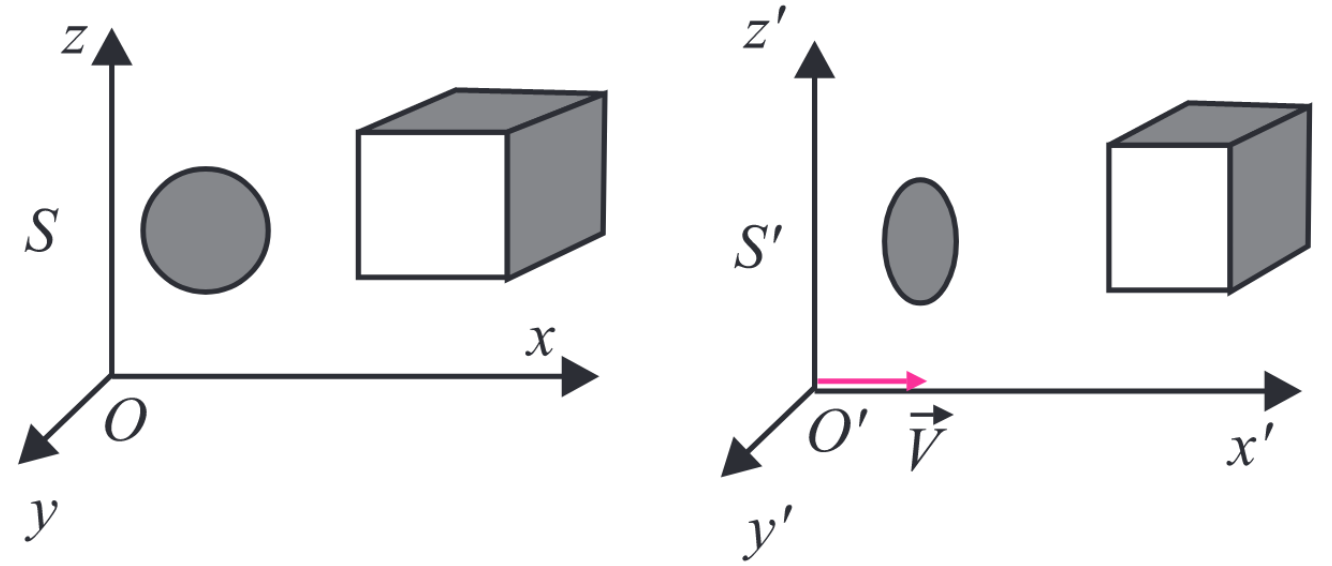
\includegraphics[width=0.4\textwidth]{fig/turtit}
    \caption{Sfera se turtește, iar cubul \linebreak se transformă în paralelipiped}
\end{wrapfigure}

Privind o sferă dintr-un sistem de referință față de care se mișcă, aceasta
apare turtită în direcția mișcării. Un cub devine un paralelipiped.

Aceste modificări reprezintă forma reală a obiectelor, nu doar ceea ce vede un
observator. Atunci când observăm un obiect în mișcare rapidă, în realitate
înregistrăm fotonii care ajung pe retină. Fotonii nefiind emiși
simultan de toate punctele corpului, ochiul percepe o imagine deformată.

Dacă viteza corpului ar fi \( V = c \), dimensiunea sa longitudinală s-ar reduce
la zero, corpul degenerând într-un plan transversal față de $Ox$.

Prin urmare, concepția spațiului absolut \( \left( l' = l_0 \right) \) este
înlocuită în teoria relativistă de concepția spațiului relativ, reprezentată
de relația \( l' = l_0 \lorentzradical \). Orice dimensiune poate fi cunoscută
numai în mărime relativă.

Pentru \( V \rightarrow 0 \), avem \( \lorentzradical \rightarrow 1 \) și deci
relația clasică \( l' = l_0 \).

Pentru \( V > c \), radicalul lui Lorentz devine imaginar, iar noțiunea de lungime
își pierde sensul.

\pagebreak

\subsection{Dilatarea relativistă a timpului}
Pe semiaxa $Ox$ a sistemului $S$, considerăm un eveniment temporar cu durata
\[ \tau_0 = t_2(x) - t_1(x) \]

$\tau_0$ mai este numit și timp propriu.

Durata acestui eveniment, măsurată în sistemul $S'$, aflat în mișcare față de
$S$, este egală cu diferența momentelor respective în $S'$ luate pentru aceeași
abscisă $x$:
\[ \tau' = t_2'(x) - t_1'(x) \]

Din \( t' = \dfrac{t - \frac{Vx}{c^2}}{\lorentzradical} \) rezultă:
\[
    \tau'
    = \frac{t_2 - \frac{Vx}{c^2}}{\lorentzradical}
    - \frac{t_1 - \frac{Vx}{c^2}}{\lorentzradical}
    = \frac{t_2 - t_1}{\lorentzradical} = \frac{\tau_0}{\lorentzradical} > \tau_0
\]

Prin urmare, durata $\tau'$ măsurată în sistemul $S'$ a unui eveniment într-un
punct aflat în mișcare față de $S'$ este mai mare decât durata $\tau_0$
măsurată în sistemul $S$, față de care punctul se află în repaus:
\( \tau' > \tau_0 \).

De aici rezultă că durata unui eveniment este minimă măsurată față de sistemul
de referință propriu.

\parbreak

%Dependența intervalului de timp de sistemul de referință nu este intuitivă în
%comparație cu fenomenele pe care le observăm zi de zi în regim nerelativist,
%când \( V \ll c \).
%
%Un exemplu îl reprezintă prezența miuonilor la nivelul solului sau mării.
%Miuonii, care apar în atmosferă la altitudini de 10 km, datorită razelor
%cosmice ce pătrund în atmosfera planetei, au un timp de viață propriu -- cel
%măsurat în SRP -- extrem de scurt, \( \tau_0 = 2,2 \cdot 10^{-6} ~ \mathrm{s} \).
%Având viteza \( V = 2,994 \cdot 10^8 \) m/s (valoare apropiată de viteza
%luminii), din calculul nerelativist al distanței rezultă că un miuon ar putea
%parcurge doar \( V\tau_0 = 658,7 \) m în intervalul de timp propriu, distanță
%insuficientă pentru a ajunge la nivelul solului.  Deoarece observația se face
%în raport cu Pământul, trebuie să luăm în considerație intervalul de timp
%măsurat față de Pământ:
%
%\[
%    \tau = \frac{\tau_0}{\lorentzradical}
%    = \frac{2,2 \cdot 10^{-6}}{\sqrt{1 - \left( \frac{2,994}{2,9979} \right)^2}}
%    = 43,14 \cdot 10^{-6} ~ \mathrm{s}
%\]
%
%Calculând acum distanța parcursă de miuon față de Pământ, obținem:
%\[ D = c\tau = 12,933 ~ \mathrm{km} \]
%
%Rezultă că miuonul poate fi reperat la nivelul solului și chiar al mării.

Pentru \( V \ll c \) se obține \( \tau = \tau_0 \), ca în mecanica clasică.

Pentru \( V \rightarrow c \), dimensiunile longitudinale ale corpurilor tind
către 0, iar intervalul de timp către infinit.

Pentru \( V = c \), corpul este redus la un plan transversal pe direcția
mișcării, iar intervalul de timp devine infinit.

Pentru \( V > c \), transformările Lorentz devin imaginare și își pierd
sensul fizic, demonstrând că viteza luminii în vid nu poate fi atinsă de
corpuri.

În concluzie, pentru un observator aflat în mișcare față de locul unde se
produce un fenomen, acesta se desfășoară mai lent decât pentru un observator
aflat în repaus față de eveniment.

Simultaneitatea a două evenimente este de asemenea dependentă de sistemul de
referință față de care este descrisă mișcarea. Două evenimente simultane în
$S$ nu sunt simultane în $S'$.

Fie două evenimente simultane în $S$ în punctele $x_1$ și $x_2$ la momentul
$t$. În $S'$, aflat în mișcare față de $S$, vom măsura timpii:
\begin{equation*}
    \begin{aligned}[t]
        t_1'(x_1) = \frac{t - \frac{Vx_1}{c^2}}{\lorentzradical}
    \end{aligned}
    \qquad\qquad\qquad
    \begin{aligned}[t]
        t_2'(x_2) = \frac{t - \frac{Vx_2}{c^2}}{\lorentzradical}
    \end{aligned}
\end{equation*}

Observate din $S'$, evenimentele nu mai apar simultane, cu excepția cazului în
care \( x_1 = x_2 \), adică atunci când evenimentele coincid.

Rolul principal al teoriei relativității este de a stabili
\emph{invarianții relativiști}: mărimi cu proprietatea de a rămâne invariante
la trecerea de la un SRI la altul. Printre aceștia se numără constantele
universale, sarcina electrică, mărimile măsurate față de SRP etc.



\section{Ipoteza de Broglie. Difracția electronilor. Aplicații}

Analog cu dualismul undă-corpuscul în cazul undelor electromagnetice, Louis de Broglie asociază oricărei microparticule în mișcare cu energia $E$ și impulsul $p$ o undă caracterizată prin frecvența $\nu$ și lungimea de undă $\lambda$, cu relațiile dintre mărimi
\[
    E = h \nu
    \begin{Bmatrix}
        \nu & \lambda \\
        E   & p
    \end{Bmatrix}
    p = \frac{h}{\lambda}
\]

De Broglie a presupus că lungimea de undă a undelor asociate microparticulelor
trebuie să fie dată tot de relația \( \lambda = \frac{h}{p} \), unde $p$ este
impulsul microparticulei.

\parbreak

Ipoteza de Broglie afirmă că oricărei microparticule care posedă un impuls $p$
i se poate asocia în mod formal o undă cu lungimea de undă
\( \lambda_B = \frac{h}{p} \), numită lungime de undă de Broglie.

Undelor electromagnetice le sunt asociați fotonii, care nu au masă de repaus.
Analog, undele de Broglie sunt asociate particulelor cu masă de repaus:
electroni, protoni, neutroni, particule \alpha, molecule de hidrogen. În
concluzie, radiația electromagnetică are proprietăți ondulatorii și
corpusculare, asemenea radiației corpusculare.

\subsection*{Experimentul Davisson-Germer}

Fizicienii Davisson și Germer au confirmat experimental ipoteza de Broglie,
demonstrând că electronii în mișcare prezintă proprietăți ondulatorii, prin
generarea fenomenelor de difracție însoțite de interferență.

\begin{wrapfigure}{r}{0.45\textwidth}
    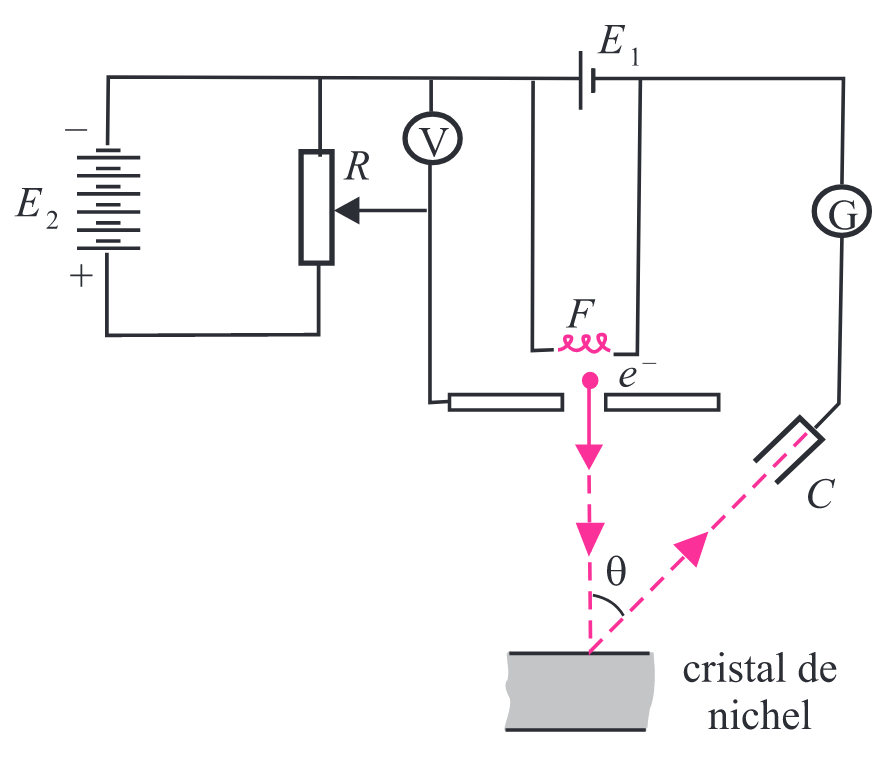
\includegraphics[width=0.45\textwidth]{fig/davisson_germer}
    \caption{Schema experimentului}
\end{wrapfigure}

Filamentul $F$, alimentat de sursa $E_1$, emite electroni care sunt accelerați
într-un tun electronic, alimentat de sursa $E_2$. Tensiunea de accelerare $U$
este controlată de reostatul $R$ și măsurată cu voltmetrul $V$.

Fasciculul monoenergetic de electroni, numit \emph{monocromatic}, care iese din
tunul electronic, are energia:
\begin{equation}
    \frac{m_e v^2}{2} = eU \label{eq:1}
\end{equation}

Fasciculul cade pe un monocristal de nichel, iar fasciculul difractat este
captat de un cilindru Faraday $C$ colector. Curentul de electroni este măsurat
de galvanometrul $G$.

Se observă că intensitatea fasciculului de electroni difractați prezintă maxime
și minime în funcție de $U$ și unghiul de incidență $\theta$.

Din relația \eqref{eq:1} rezultă \( v = \sqrt{\frac{2eU}{m_e}} \).

În cazul nerelativist avem impulsul \( p = m_e v = \sqrt{2em_e U} \), iar
lungimea de undă de Broglie asociată este:
\[
    \lambda_B = \frac{h}{p} = \frac{h}{\sqrt{2em_e} U}
    = \frac{h}{\sqrt{2em_e}} \cdot \frac{1}{\sqrt{U}}
    = \frac{12,23 \cdot 10^{-10}}{\sqrt{U}}
\]

Pentru un potențial de accelerare \( V = 54 \unit{V} \), lungimea de undă
este de același ordin de mărime cu lungimea de undă a radiației X:
\begin{equation}
    \lambda_B = \frac{12,23 \cdot 10^{-10}}{\sqrt{54}}
    = 1,664 \cdot 10^{-10} \unit{m} \label{eq:2}
\end{equation}

Fenomenele de difracție pot fi observate când unda interacționează cu o „rețea
de difracție” a cărei constantă de rețea are dimensiunile comparabile cu
lungimea de undă (\( 10^{-10} \unit{m} \)).

\begin{wrapfigure}{r}{0.45\textwidth}
    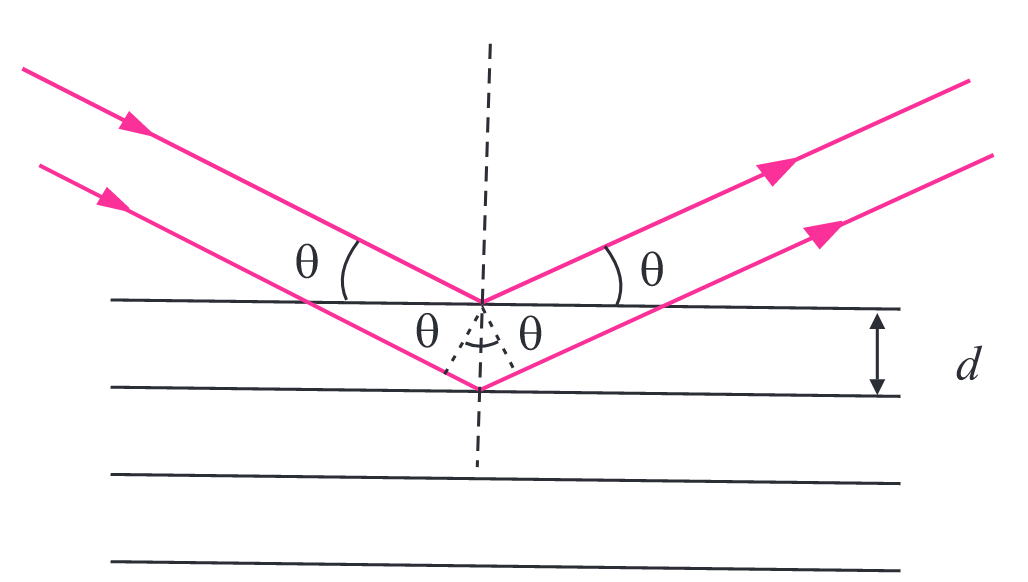
\includegraphics[width=0.45\textwidth]{fig/monocristal}
    \caption{Difracția razelor X pe un monocristal}
\end{wrapfigure}

Atomii monocristalului sunt așezați ordonat, distanța dintre doi atomi vecini
fiind de ordinul \( 10^{-10} \unit{m} \). Această aranjare regulată în nodurile
rețelei cristaline conferă proprietățile unei rețele de difracție
tridimensionale.

În urma studierii difracției razelor X pe monocristale, Bragg a stabilit că
intensitatea fasciculului difractat trece prin valori maxime în cazul:
\begin{equation}
    2d\sin\theta = k\lambda, k \in \mathbb{N^*} \label{eq:3}
\end{equation}
unde:
\begin{itemize}
    \item $\theta$ este unghiul format de planul reticular cu direcția fasciculului incident, respectiv cel difractat.
    \item $d$ este constanta rețelei, adică distanța dintre două plane reticulare.
    \item $\lambda$ este lungimea de undă a radiației.
    \item $2d\sin\theta$ este diferența de drum dintre razele difractate de două plane reticulare vecine.
\end{itemize}

În cazul în care particulele suferă o difracție, se aplică relația
\eqref{eq:3}. Pentru \( d = 0,91 \cdot 10^{-10} \unit{m} \), $k = 1$,
$U = 54 \unit{V}$, tensiune la care se obține primul maxim pentru
$\theta = 65^\circ$, se obține:
\begin{equation}
    \lambda_B = 2d\sin\theta = 2 \cdot 0,91 \cdot 10^{-10} \cdot 0,906 = 1,65 \cdot 10^{-10} \unit{m} \label{eq:4}
\end{equation}

Valorile obținute în relațiile \eqref{eq:2} și \eqref{eq:4} se află în concordanță, confirmând că
electronii în mișcare au proprietăți ondulatorii.

Lungimea de undă de Broglie este invers proporțională cu masa particulelor cărora le este asociată.

Microparticulele, numite \emph{particule cuantice}, sunt radical diferite de
particulele clasice, supunându-se unor legi specifice. Nu sunt nici particule,
nici unde în sens clasic, comportamentul lor reflectând dualismul
corpuscul-undă.

Deși unda de Broglie asociată microparticulelor nu este o undă în sensul clasic
al cuvântului, este folosită această noțiune.

La nivel macroscopic, un corpuscul nu poate avea proprietăți ondulatorii, iar
unda nu poate fi concepută ca un flux de particule discrete. Particulele
cuantice aparțin însă nivelului cuantic, fiind radical diferite de unde și
corpusculi. De exemplu, ele nu au traiectorii.

Asupra sistemelor cuantice putem face doar afirmații statistice.

\subsection*{Microscopul electronic}

Microscopul electronic este o aplicație a ipotezei lui de Broglie. Un
fasciculul de electroni cade pe un preparat și îl traversează, variațiile de
grosime ale preparatului devenind variații de intensitate a fasciculului.
Utilizând câmpuri electrice sau magnetice, traiectoriile electronilor sunt
asemănătoare traiectoriilor razelor de lumină dintr-un microscopic optic.

În cazul microscopului optic, pentru a distinge două puncte, distanța dintre
ele trebuie să fie mai mare decât lungimea de undă a luminii folosite, adică
mai mare decât zecimi de microni (puterea de separare).

În locul lentilelor optice se găsesc bobinele parcurse de curent electric
(\emph{lentile magnetice}) sau electrozii încărcați electric
-- \emph{lentile electrice} -- ce pot focaliza și defocaliza un fascicul de
electroni.

\parbreak

\begin{minipage}{0.6\textwidth}
    \captionsetup{type=figure}
    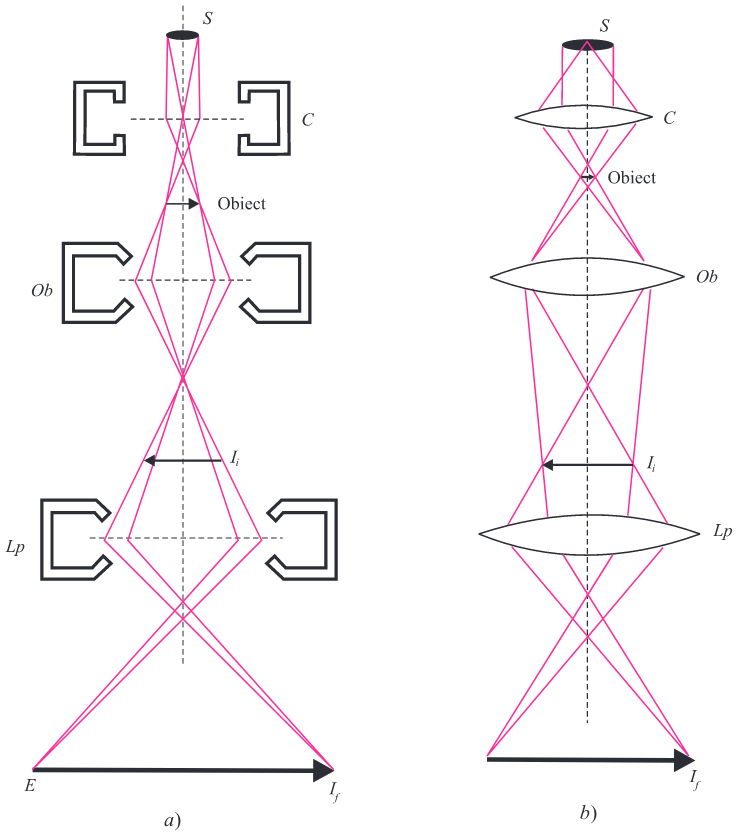
\includegraphics[width=\textwidth]{fig/microscop}
    \caption{Schema microscopului electronic și a microscopului optic}
\end{minipage}%
\hspace{0.5cm}%
\begin{minipage}{0.3\textwidth}
    \begin{itemize}[left=0pt,label=]
        \item $S$ -- sursa de electroni (a) sau lumină (b)
        \item $C$ -- condensator
        \item $Ob$ -- obiectiv
        \item $I_i$ -- imagine intermediară
        \item $Lp$ -- lentilă de proiecție
        \item $I_f$ -- imagine finală
        \item $E$ -- ecran fluorescent
    \end{itemize}
\end{minipage}

\parbreak

Datorită lungimii de undă mult mai mici a undelor asociate electronilor,
puterea de separare a microscopului electronic este mult mai mare decât a
microscopului optic. Transformarea imaginii în una luminoasă se realizează cu
ajutorul unui ecran fluorescent.

Probele examinate trebuie să fie sub formă de pelicule foarte subțiri, din
cauza puterii de pătrundere mici a electronilor.

Au fost construite și microscoape protonice și ionice, care pot mări de 10-15
ori mai mult decât un microscop electronic.

\section{Modelul Bohr}

Ideea corectă a modelului Rutherford de existență a unui nucleu atomic în care
este concentrată aproape toată masa și toată sarcina pozitivă a atomului a fost
preluată în modelele atomice propuse ulterior.

În conceptul lui Bohr, atomul este un sistem solar în miniatură, cu forțe
electrice în loc de forțe gravitaționale. Nucleul încărcat pozitiv joacă rolul
soarelui, iar electronii se mișcă în jurul lui sub acțiunea forțelor electrice
de atracție.

Acest model atomic se bazează pe \emph{postulatele lui Bohr}.

În fizica clasică, energia unui sistem poate varia în mod continuu.

Având o masă mai mică decât a atomilor, electronii nu vor pierde energie la o
ciocnire, ci vor fi \emph{împrăștiați elastic}. Însă în urma unei ciocniri
inelastice cu un atom, electronul va pierde energie, iar viteza lui va scădea.
Energia pierdută va fi transferată atomului ciocnit, care trece într-o
\emph{stare excitată}. Se constată, pe cale experimentală, că atomul poate
primi energie numai în anumite valori bine determinate.
\emph{Atomul poate avea numai anumite stări (discrete) de energie}.

\emph{Cuanta} de radiație este unitatea structurală de bază a câmpurilor ce
poate fi emisă sau absorbită de un sistem fizic (molecular, atomic, nuclear
etc.). De exemplu, fotonul pentru câmpul electromagnetic. Energia unei cuante
de radiație se mai numește \emph{cuantă de energie}.

\emph{Cuantificarea} este procedeul mecanicii cuantice prin care se impune ca
mărimile fizice ce caracterizează sistemul de particule să ia doar valori
discrete. De exemplu, energia, impulsul, momentul cinetic etc.

S-a constatat că intensitatea și frecvența radiației emise cresc odată cu
energia de excitare, raportul energie-frecvență fiind constanta lui Planck
(numită și \emph{cuantă de acțiune}):
\[ \frac{E}{\nu} = h = 6,626075 \cdot 10^{-34} ~ \mathrm{J \cdot s} \]

Se poate scrie că energia radiațiilor emise de atomii care se dezexcită este
proporțională cu frecvența:
\[ E = h\nu \]

În conceperea modelului cuantificat, au fost emise cele două postulate ale lui
Bohr:
\begin{enumerate}[label=\Roman*.]
    \item Atomii și sistemele atomice se pot găsi timp îndelungat numai în
        stări bine determinate, numite stări staționare, în care nu emit și nu
        absorb energie. \\
        Energia sistemului în aceste stări este cuantificată, adică ia valori
        ce alcătuiesc un șir discontinuu: \( E_1, E_2, ..., E_n \).
    \item Atomii emit sau absorb radiație electromagnetică doar la trecerea
        dintr-o stare staționară $m$, caracterizată de energia $E_m$, în altă
        stare staționară $n$, caracterizată de energia $E_n$. \\
        Frecvența radiației emise sau absorbite într-o astfel de tranziție este
        dată de relația:
        \[ h\nu_{mn} = E_m - E_n \]
        Acest postulat explică spectrele de linii ale radiațiilor emise de
        atomii de hidrogen.
\end{enumerate}

\subsection{%
    Cuantificarea distanțelor electronului față de nucleu%
    \texorpdfstring{ ($r_n$)}{}, a vitezelor lui pe orbita
    circulară\texorpdfstring{ ($v_n$)}{}, a impulsului%
    \texorpdfstring{ ($p_n$)}{}, și a energiei totale%
    \texorpdfstring{ ($E_n$)}{}
}

Aceste mărimi pot fi obținute considerând că forța coulombiană este o forță de
natură centripetă:
\begin{equation}
    \frac{e^2}{4\pi\varepsilon_0 r^2} = \frac{mv^2}{r}
    \label{eq:2}
\end{equation}
și că electronului i se poate asocia o undă cu lungimea de undă
\( \lambda_B = \frac{h}{p} \).

Pot exista numai acele orbite ale electronului în atom pentru care este
satisfăcută condiția existenței undelor de Broglie staționare. Pentru aceasta,
lungimea orbitei circulare trebuie să cuprindă un număr întreg de lungimi de
undă, adică exact \emph{condiția de cuantificare a momentului cinetic al
mișcării electronului pe o orbită staționară}:
\[ 2\pi r = n\lambda_B = \frac{nh}{mv} \]
\begin{center}
    sau
\end{center}
\begin{equation}
    mvr = n\frac{h}{2\pi} = n\overline{h}, ~ n \in \mathbb{N}^*
    \label{eq:3}
\end{equation}
unde $\overline{h}$ se numește constanta Planck redusă (sau constanta Dirac).

\begin{wrapfigure}{l}{0.4\textwidth}
    \centering
    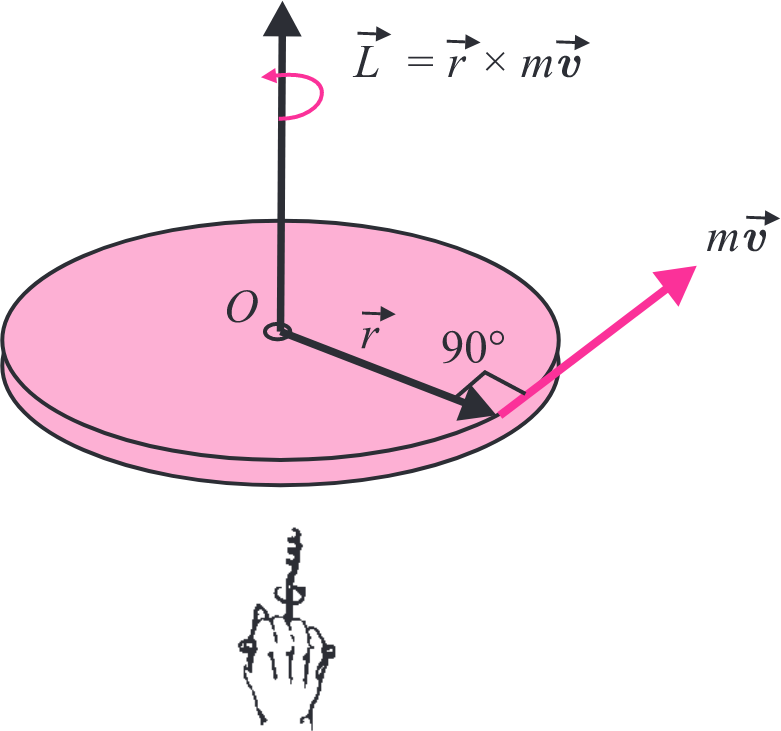
\includegraphics[width=0.35\textwidth]{fig/moment_cinetic}
    \caption{Momentul cinetic al punctului material în mișcarea circulară}
\end{wrapfigure}

\emph{Momentul cinetic} (sau \emph{moment al impulsului}) $\vec{L}$ este
analogul impulsului în mișcarea de rotație. Este definit ca produsul vectorial
dintre vectorul de poziție $\vec{r}$ al originii vectorului impuls, față de
centrul de rotație, și impulsul punctului material $\vec{p} = m\vec{v}$:
\[ \vec{L} = \vec{r} \times \vec{p} = \vec{r} \times m\vec{v} \]

Momentul cinetic este un vector cu modulul \( L = rp\sin(\vec{r}, m\vec{v}) \).
În mișcarea circulară, \( \vec{r} \perp m\vec{v} \), deci $L = rmv$. Se măsoară
în SI în kg \cdot\ m$^2$s$^{-1}$ = J \cdot s.

\clearpage

Postulatele lui Bohr nu decurg din niciun principiu al fizicii clasice, ci se
bazează doar pe fizica cuantică. Conform condiției de cuantificare a lui Bohr,
electronul se poate mișca în jurul nucleului doar pe acele orbite pentru care
$L$ este un multiplu al lui $\overline{h}$.

Din relațiile \eqref{eq:2} și \eqref{eq:3} pot fi deduse expresiile
cuantificate ale $r_n$, $v_n$, $p_n$, $E_n$:
\begin{align*}
    \frac{e^2}{4\pi\varepsilon_0 r^2} = \frac{mv^2}{r}
    &\Rightarrow v^2 = \frac{e^2}{4\pi\varepsilon_0 rm}
    \\
    rmv = n\frac{h}{2\pi} &\Rightarrow v^2 = \frac{n^2 h^2}{4\pi^2 m^2 r^2}
    \Rightarrow \boxed{v_n = \frac{nh}{2\pi mr_n}}
\end{align*}

Din aceste două exprimări ale $v^2$ rezultă
\( \frac{e^2}{4\pi\varepsilon_0 rm} = \frac{n^2 h^2}{4\pi^2 m^2 r^2} \), de
unde se obține:
\[
    \boxed{r_n = \frac{\varepsilon_0 h^2}{\pi me^2} n^2}
    \Rightarrow \boxed{v_n = \frac{e^2}{2\varepsilon_0 h} \frac{1}{n}}
\]
\[
    p_n = mv^n \Rightarrow
    \boxed{p_n = \frac{me^2}{2\varepsilon_0h} \frac{1}{n}}
\]

Din \eqref{eq:1} se obține:
\begin{equation}
    E_n = -\frac{e^2}{8\pi\varepsilon_0 r_n}
    \Rightarrow \boxed{E_n = -\frac{me^4}{8\varepsilon_0^2 h^2} \frac{1}{n^2}}
    \label{eq:4}
\end{equation}

Aplicăm expresiile deduse atomului de hidrogen $^1_1$H.
Pentru $n = 1$, raza primei orbite Bohr este:
\begin{equation}
    r_1 = \frac{\varepsilon_0 h^2}{\pi m e^2}, ~\text{iar}~ r_n = r_1n^2
    \label{eq:5}
\end{equation}
Orbitele neradiante permise au deci razele $r_1$, $4r_1$, $9r_1$ etc.

Știind
\begin{align*}
    \varepsilon_0 &= \SI{8,85d-12}{\coulomb\tothe{2}\per\newton\per\metre\tothe{2}}
    \hspace{0.75cm}
    &h &= \SI{6,62d-34}{\joule\cdot\second}
    \\
    m &= \SI{9,11d-31}{\kilogram}
    \hspace{0.75cm}
    &e &=\SI{1,60d-19}{\coulomb}
\end{align*}
se obține \( r_1 = \SI{0,53d-10}{\metre} \), valoare aflată în concordanță cu
diametrele atomice estimate prin alte metode.

Conform \eqref{eq:5}, distanța dintre două orbite consecutive crește odată cu
îndepărtarea de nucleu.

Orice sistem fizic tinde spre starea echilibru stabil, care corespunde energiei
cele mai joase. Energia sistemului nucleu-electron fiind negativă, starea
energetică cea mai joasă se atinge când această energie are valoarea absolută
cea mai mare, deci pentru $n = 1$.

Această stare, de energie minimă, se numește \emph{stare fundamentală} sau
\emph{normală}.

În cazul atomului de hidrogen, din relația \eqref{eq:4} rezultă:
\[ E_1 = -\frac{me^4}{8h^2\varepsilon_0^2} = \SI{-13,6}{\electronvolt} \]

\begin{wrapfigure}{l}{0.45\textwidth}
    \centering
    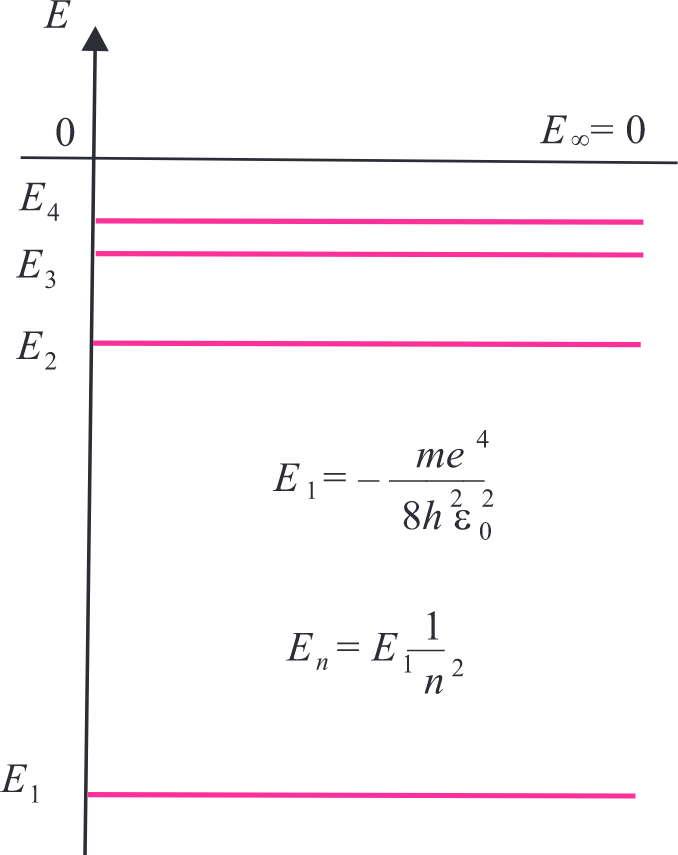
\includegraphics[width=0.4\textwidth]{fig/niveluri_energie_hidrogen}
    \caption{Nivelurile de energie ale atomului de hidrogen}
\end{wrapfigure}

În fig. 7, liniile orizontale indică \emph{nivelurile de energie} (valorile
energiei totale).

Originea se află în $E = 0$, pentru numere cuantice foarte mari, când
electronul este depărtat de nucleu și pierde legătura cu acesta (ionizare).

Deasupra $E = 0$ pot fi reprezentate valorile pozitive ale energiei, ce
corespund mișcării libere a electronului și care nu sunt cuantificate, fiind
posibilă orice valoare. \emph{Stările legate} ale electronului în atom sunt
exprimate prin energiile negative, reprezentate sub $E = 0$.

Se observă că nivelurile cuantificate se strâng spre 0.
\[ E_n = \frac{E_1}{n^2} \]

Relațiile deduse sunt aplicabile atomului de hidrogen și atomilor hidrogenoizi
(cu un singur electron): He$^+$ (o dată ionizat), Li$^{++}$ (de două ori
ionizat), Be$^{+++}$ (de trei ori ionizat) etc.

În general, pentru atomii hidrogenoizi, unde $Z$ este numărul atomic:
\[
    E_n = -\frac{mZ^2e^4}{8h^2\varepsilon_0^2}
    = -13,6 \cdot \frac{Z^2}{n^2} ~ \si{\electronvolt}
\]

\subsection{Seriile spectrale ale hidrogenului și ale atomilor hidrogenoizi}

Electronul poate trece din starea fundamentală într-o stare excitată prin
absorbția unui foton. Această stare excitată nu este stabilă.

Un atom se dezexcită în \SI{d-8}{\second}, energia înmagazinată fiind radiată
sub formă de energie a unei unde electromagnetice de frecvență bine
determinată, acoperind întregul domeniu spectral, de la infraroșu la
ultraviolet.

Energia fotonului emis sau absorbit la trecerea de la o stare staționară la
alta este dată de postulatul al II-lea al lui Bohr.

Urmează studiul spectrelor de emisie -- trecerea electronului dintr-o stare
excitată într-o stare de energie mai joasă, la emiterea unui foton de energie
$h\nu$ (prin dezexcitare).

Ne vom referi la spectrul de emisie al atomului de hidrogen (H), care este un
spectru de linii.

Fie $n-i$ numărul cuantic al unei stări excitate oarecare, și $n_f$ numărul
cuantic al stării de energie mai joase, pe care se întoarce electronul după
emisie.

Energia inițială este:
\[ E_i = -\frac{me^4}{8\varepsilon_0 h^2} \frac{1}{n_i^2} \]

Energia finală este:
\[ E_f = -\frac{me^4}{8\varepsilon_0 h^2} \frac{1}{n_f^2} \]

Energia fotonului emis, $h\nu$, va fi egală cu:
\[
    E_i - E_f = h\nu
    = -\frac{me^4}{8\varepsilon_0 h^2} \frac{1}{n_i^2}
    + \frac{me^4}{8\varepsilon_0 h^2} \frac{1}{n_f^2}
\]

Frecvența liniei emise, $\nu$, va fi:
\[
    \nu = \frac{me^4}{8\varepsilon_0 h^2}
    \left(\frac{1}{n_f^2} - \frac{1}{n_i^2}\right)
\]

Introducem notația pentru \emph{numărul de undă} $\tilde{\nu}$ -- numărul de
lungimi de undă cuprinse în intervalul unitate:
\[ \tilde{\nu} = \frac{\nu}{c} = \frac{1}{cT} = \frac{1}{\lambda} \]

Atunci:
\[
    \tilde{\nu} = \frac{me^4}{8\varepsilon_0 h^2}
    \left(\frac{1}{n_f^2} - \frac{1}{n_i^2}\right)
\]

Mărimea $\frac{me^4}{8\varepsilon_0 h^2}$ este \emph{constanta lui Rydberg},
având valoarea $R = \SI{1,097373d7}{\per\meter}$.

Astfel, energia cuantificată a electronului pe un nivel energetic al atomului
poate fi exprimată ca:
\[ \boxed{E_n = -\frac{Rch}{n^2}} \]

Grupul de linii spectrale cu același $n_f$ formează o \emph{serie spectrală}.

Pentru $n_i \rightarrow \infty$, numărul de undă este maxim, cu valoarea
$\frac{R}{n^2}$, numită limita seriei.

\emph{Inversele lungimilor de undă ale liniilor spectrale emise de atomul de
hidrogen} sunt date de ecuația:
\[ \tilde{\nu} = R \left(\frac{1}{n_f^2} - \frac{1}{n_i^2}\right) \]
iar pentru \emph{atomii hidrogenoizi}, cu sarcina $Ze$ și un singur electron,
de ecuația:
\[ \tilde{\nu} = RZ^2 \left(\frac{1}{n_f^2} - \frac{1}{n_i^2}\right) \]

\clearpage

\begin{wrapfigure}{r}{0.45\textwidth}
    \centering
    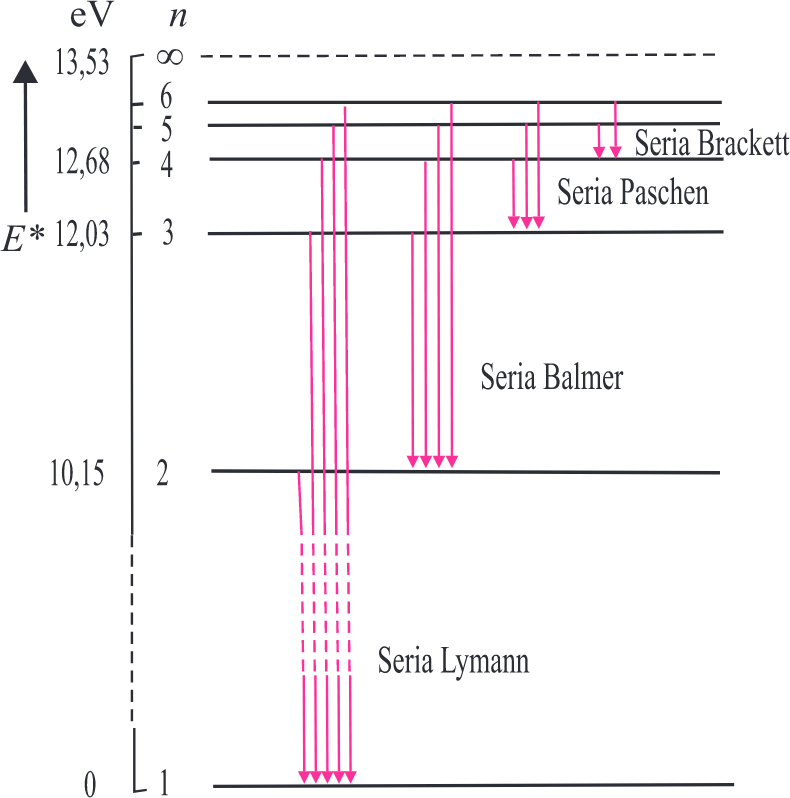
\includegraphics[width=0.4\textwidth]{fig/tranzitii_electron}
    \caption{Tranzițiile electronului în modelul Bohr al atomului de hidrogen}
\end{wrapfigure}

Cu mult înainte ca Bohr să elaboreze modelul atomic al hidrogenului, studiind
liniile din vizibil ale atomului, Balmer a observat că lungimile de undă ale
liniilor spectrale emise respectă anumite regularități.

Rydberg a rearanjat \emph{relația empirică a lui Balmer}, pentru calculul
lungimilor de undă:
\[ \tilde{\nu} = \frac{1}{\lambda} = R\left(\frac{1}{2^2} - \frac{1}{n^2\right}) \]

S-a obținut empiric aceeași valoare a lui $R$ ca în modelul atomic al lui Bohr.

Seriile spectrale ale hidrogenului sunt redate în tabelul următor.

Tranzițiile sunt ilustrate în fig. 8, și pot fi realizate direct sau în trepte.
Numărul tranzițiilor posibile este egal cu $C_n^2 = \frac{(n-1)n}{2}$.

\begin{center}
    \renewcommand{\arraystretch}{1.5}
    \begin{tabular}{|c|c|c|c|c|}
        \hline
        \textbf{Denumirea seriei spectrale} & \boldmath$n_f$ & \boldmath$n_i$ &
        \textbf{Domeniul spectral} & \textbf{Limita seriei} \\
        \hline
        Lyman & 1 & 2, 3, ... & ultraviolet & $R$ \\
        \hline
        Balmer & 2 & 3, 4, ... & vizibil & $R/4$ \\
        \hline
        Paschen & 3 & 4, 5, ... & infraroșu & $R/9$ \\
        \hline
        Brackett & 4 & 5, 6, ... & infraroșu & $R/16$ \\
        \hline
        Pfund & 5 & 6, 7, ... & infraroșu îndepărtat & $R/25$ \\
        \hline
    \end{tabular}
\end{center}

\subsection*{Aplicații ale spectroscopiei}

Spectroscopia este o metodă comodă, precisă, și rapidă în analiza chimică, cu
ajutorul acesteia fiind descoperite elementele cesiu, taliu, indiu, și galiu.

Sursele moderne de iluminare, precum tuburile cu descărcare rapidă în vapori de
sodiu sau mercur, sau lămpile fluorescente, au fost inventate pe baza studiilor
spectroscopice.

Ceasul atomic este instrumentul de măsurare a timpului cel mai precis, utilizat
de exemplu la GPS. O secundă este egală cu 9192631770 perioade asociate
tranziției între două niveluri energetice ale cesiului 133.

Cele mai importante utilizări ale spectroscopiei au avut loc în astronomie, în
studiul temperaturii, compoziției, și deplasării astrelor.

\clearpage
\section{Relația masă-energie}

În teoria relativității restrânse sunt valabile și teoremele rezultate
din principiul fundamental al mecanicii \( \vec{F} = \diff{(m\vec{v})}{t} \),
printre care se află și teorema variației energiei cinetice.

Din
\[
    \dd E_c = \dd L = \vec{F}\dd\vec{r}
    \hspace{3cm}
    \vec{F} = \diff{(m\vec{v})}{t}
    \hspace{3cm}
    \dd\vec{r} = \vec{v} \dd t
\]
rezultă:
\begin{align*}
    \dd E_c &= \diff{(m\vec{v})}{t} \vec{v}\dd t = \vec{v} \dd(m\vec{v}) \\
            &= \vec{v} (m\dd\vec{v} + \vec{v} \dd m) \\
            &= m\vec{v}\dd\vec{v} + v^2 \dd m \\
            &= mv \dd v + v^2 \dd m
\end{align*}

Folosind relația $m(v)$ aflată anterior, se obține:
\begin{align*}
    \dd m &= \diff{m}{v} \dd v = \frac{\dd}{\dd v} \left(\frac{m_0}{\lorentzradical}\right) \dd v \\
          &= \frac{-m_0 \left(-\frac{2v}{2c^2\lorentzradical}\right)}{1 - \frac{v^2}{c^2}} \\
          &= \frac{m_0}{\lorentzradical} \cdot \frac{\frac{v}{c^2}}{\left(1 - \frac{v^2}{c^2}\right)} \cdot\dd v \\
          &= m \cdot \frac{v}{c^2 - v^2} \cdot\dd v = \frac{mv \dd v}{c^2 - v^2}
\end{align*}
de unde rezultă: \( mv \dd v = (c^2 - v^2) \dd m \). Înlocuind în relația anterioară, rezultă:
\[ \dd E_c = (c^2 - v^2) \dd m + v^2 \dd m = c^2 \dd m \]

Integrăm de la masa de repaus $m_0$ (când $E_{c_0}$, $v_0 = 0$) la masa de mișcare $m(v)$:
\[ E_c = c^2 \int\limits_{m_0}^m \dd m = mc^2 - m_0c^2 \]

Altfel spus: \( E_c = E - E_0 \), unde \( E = mc^2 \) este energia totală
relativistă asociată masei de mișcare, iar \( E_0 = m_0c^2 \) energia
totală relativistă asociată masei de repaus.

Unei creșteri infinit de mici a masei îi corespunde o energie cinetică
finită, datorată factorului foarte mare \( c^2 = 9 \cdot 10^{16} ~ \mathrm{m^2/s^2} \).

Sub altă formă:
\[ E_c = (m - m_0) c^2 = \left( \frac{1}{\lorentzradical} - 1 \right) m_0c^2 \]

Folosind dezvoltarea în serie Taylor:
\[ f(x) = f(0) + \frac{1}{1!}f'_x(0) + \frac{1}{2!}f''_x(0) x^2 + ...\]
a funcției \( \frac{1}{\sqrt{1-x}} \), după puterile raportului \( x = \frac{v^2}{c^2} \),
și reținând primii termeni:
\begin{align*}
    f(x)   &= \frac{1}{\sqrt{1-x}} = (1 - x)^{-\frac{1}{2}}
           & f(0)   &= 1 \\
    f'(x)  &= \left(-\frac{1}{2}\right) (1 - x)^{-\frac{3}{2}}(-1) = \frac{1}{2}(1 - x)^{-\frac{3}{2}}
           & f'(0)  &= \frac{1}{2} \\
    f''(x) &= \frac{1}{2} \left(-\frac{3}{2}\right) (1 - x)^{-\frac{5}{2}}(-1) = \frac{3}{4}(1 - x)^{-\frac{5}{2}}
           & f''(0) &= \frac{3}{4} \\
\end{align*}
obținem:
\[ E_c = \left[ \left( 1 + \frac{1}{2}\cdot\frac{v^2}{c^2} + \frac{3}{8}\cdot\frac{v^4}{c^4} + ... \right) - 1 \right] m_0c^2 \]

Dacă reținem un singur termen, obținem expresia clasică a energiei cinetice:
\[ E_c \approx \frac{m_0v^2}{2} \]

Celebra formulă a lui Einstein, pe baza căreia s-a dezvoltat fizica nucleară
după anul 1905, este expresia energiei totale a particulei libere:
\[ E = mc^2 = \frac{m_0c^2}{\lorentzradical} \]

Formula aceasta a fost dedusă de fizicianul Friedrich Hasenohrl în 1904,
din considerații nerelativiste.

Deși este numită de obicei energia totală, această formulă nu include energia
potențială a particulei aflată într-un câmp exterior.

Formula \( E = mc^2 \) exprimă o legătură directă, de \emph{proporționalitate},
între energie și masă.

Prin experiențe de optică fotonică și fizică nucleară, s-a demonstrat că relația
este universală, valabilă pentru \emph{orice formă de energie}. Orice variație
de energie implică o variație a masei corpului: \( \Delta E = c^2 \Delta m \).

Legea conservării energiei este și legea conservării masei.

Pentru \( v = c \), rezultă \( m \rightarrow \infty \Rightarrow E \rightarrow \infty \),
ceea ce este inadmisibil din punct de vedere fizic. Prin urmare, și din această formulă
rezultă că viteza luminii nu poate fi atinsă.

Formula lui Einstein evidențiază energia conținută în materia aflată sub formă
de substanță. Un kilogram de substanță conține o energie imensă,
\( E_0 = 9 \cdot 10^{16} ~ \mathrm{J} \), egală cu energia necesară pentru
ridicarea a $28,7$ miliarde de tone de la sol până la vârful turnului Eiffel
(aproximativ 320 m).

Uneori, relația este greșit interpretată ca exprimând transformarea materiei în
energie. Energia este însă o proprietate a materiei, deci nu are sens să afirmăm
că materia se transformă într-o proprietate a sa. Formula exprimă un proces de
transformare a materiei dintr-o formă \emph{ponderată} (substanța) într-o formă
\emph{radiantă} (câmpul), sau invers.

\emph{Defectul de masă}, o micșorare a masei ponderale, este cauza energiei imense
ce apare în reacțiile nucleare.

Un fenomen ce verifică formula lui Einstein este cel prin care un foton
$\gamma$ absorbit de un corp se transformă în două particule corpusculare (materie
ponderală): electron $e^-$ și pozitron $e^+$. Această transformare poate avea loc
doar în cazul în care energia fotonului este cel puțin egală cu de două ori
energia relativistă de repaus a electronului sau pozitronului:
\begin{align*}
    E_{min} &= hv_{min} = 2m_0c^2 = 2\cdot9,1\cdot10^{-31}\cdot9\cdot10^{16} \\
            &= 1,64\cdot10^{-13} ~ \mathrm{J} \\
            &= 1,022 ~ \mathrm{MeV} \\
\end{align*}

Din \( \frac{hc}{\lambda_{max}} = 2m_0c^2 \) ($h$ -- constanta lui Planck) rezultă:
\begin{align*}
    \lambda_{max} &= \frac{h}{2m_0c}
                  = \frac{6,62\cdot10^{-34}}{2\cdot9,1\cdot10^{-31}\cdot3\cdot10^8}
                  = 1,21\cdot10^{-12} ~ \mathrm{m} = 0,012 ~ \text{\AA}
\end{align*}

Spre comparație, \( \lambda_{verde} = 5460 ~ \text{\AA} \gg \lambda_{max} \),
deci fotonii cu lungimea de undă $\lambda_{max}$ trebuie să fie fotoni cu energii
mari, adică fotoni $\gamma$ sau fotoni neutrino. %Cei din urmă au fost postulați de
%către fizicianul Wolfgang Pauli, care în 1930 a emis ipoteza neutrinului în acord
%cu legile de conservare a energiei și a momentului cinetic la dezintegrarea beta.

\subsection{Relația dintre energia totală, impulsul și masa de repaus în teoria
relativității restrânse}
\[
    E = mc^2 = \frac{m_0c^2}{\lorentzradical}
    \hspace{3cm}
    \vec{p} = m\vec{v} \Rightarrow v^2 = \frac{p^2}{m^2}
\]
\begin{align*}
    E &= \frac{m_0c^2}{\sqrt{1 - \frac{p^2}{m^2c^2}}}
    = \frac{m_0c^2}{\sqrt{1 - \frac{p^2c^2}{(mc^2)^2}}}
    = \frac{m_0c^2}{\sqrt{1 - \frac{p^2c^2}{E^2}}} \\
    E^2 &= \frac{(m_0c^2)^2}{1 - \frac{p^2c^2}{E^2}}
    = \frac{E^2(m_0c^2)^2}{E^2 - p^2c^2} \\
\end{align*}
\[
    \Rightarrow E^2 - p^2c^2 = m_0c^2
    \Leftrightarrow E = \sqrt{p^2c^2 + m_0^2c^4}
\]

Ajungem la relația:
{
    \color{\accentcolor}
    \[ E = c\sqrt{p^2 + (m_0c)^2} \]
}

Aceasta este exprimarea energiei în funcție de impuls în mecanica relativistă,
analoagă relației \( E_c = \frac{p^2}{2m} \) din mecanica newtoniană.

Rezultatul poate fi interpretat ca o relație de unificare pentru particulele
relativiste a energiei $E$, impulsului $p$, și masei de repaus $m_0$.

Știind că fotonii au $m_0 = 0$ și \( \lambda = \frac{c}{v} \), rezultă:
\[ E_f = p_f c \Rightarrow p_f = \frac{E_f}{c} = \frac{hv}{c} = \frac{h}{\lambda} \]

Prin urmare, fotonii au impulsul \( p = mc = \frac{h}{\lambda} \) și se
deplasează cu viteza $c$ în orice sistem inerțial, oricare ar fi impulsul lor
$p$.

\subsection{Mărimi normate. Definirea regimurilor dinamice:\\ newtonian,
relativist și extrem relativist}

Pentru tratarea unitare a mișcării particulelor, se recurge la normarea
mărimilor ce caracterizează mișcarea acestora, adică raportarea vitezei
$\vec{v}$ a particulei la viteza luminii $c$ în spațiul liber, respectiv
a masei, energiei, și impulsului la expresiile corespunzătoare particulei
în repaus.
\[
\begin{aligned}
    \vec{\beta} &= \frac{\vec{v}}{c}
    \hspace{3cm}
    &\gamma    &= \frac{E}{E_0} = \frac{m}{m_0} \\
    \eta        &= \frac{E_c}{E_0}
    &\vec{\xi} &= \frac{\vec{p}}{m_0c} = \gamma\vec{\beta}
\end{aligned}
\]

Viteza luminii este o constantă universală și este considerată în modul,
astfel încât $\vec{\beta}$ și $\vec{\xi}$ sunt vectori.


Fiecare din mărimile normate se poate exprima în funcție de celelalte:
{\renewcommand{\arraystretch}{1.3}%
    \begin{center}
        \begin{tabular}{|c|c|c|c|}
            \hline
            \beta & \( (1+\eta)^{-1}(\eta^2+2\eta)^{\frac{1}{2}} \)
                  & \( (\gamma^2-1)^{\frac{1}{2}} \gamma^{-1} \)
                  & \( \xi(1+\xi^2)^{-\frac{1}{2}} \) \\
                  \hline
            \gamma & \( (1-\beta^2)^{-\frac{1}{2}} \)
                   & \( \eta + 1 \)
                   & \( (\xi^2+1)^{\frac{1}{2}} \) \\
                   \hline
            \eta & \( (1-\beta^2)^{-\frac{1}{2}} - 1 \)
                 & \( \gamma - 1 \)
                 & \( (\xi^2+1)^{\frac{1}{2}} - 1 \) \\
                 \hline
            \xi & \( (\gamma^2-1)^{\frac{1}{2}} \)
                & \( [\eta(\eta+2)]^{\frac{1}{2}} \)
                & \( \beta(1-\beta^2)^{-\frac{1}{2}} \) \\
                \hline
        \end{tabular}
    \end{center}
}

{
    \begin{wrapfigure}{r}{0.45\textwidth}
        \centering
        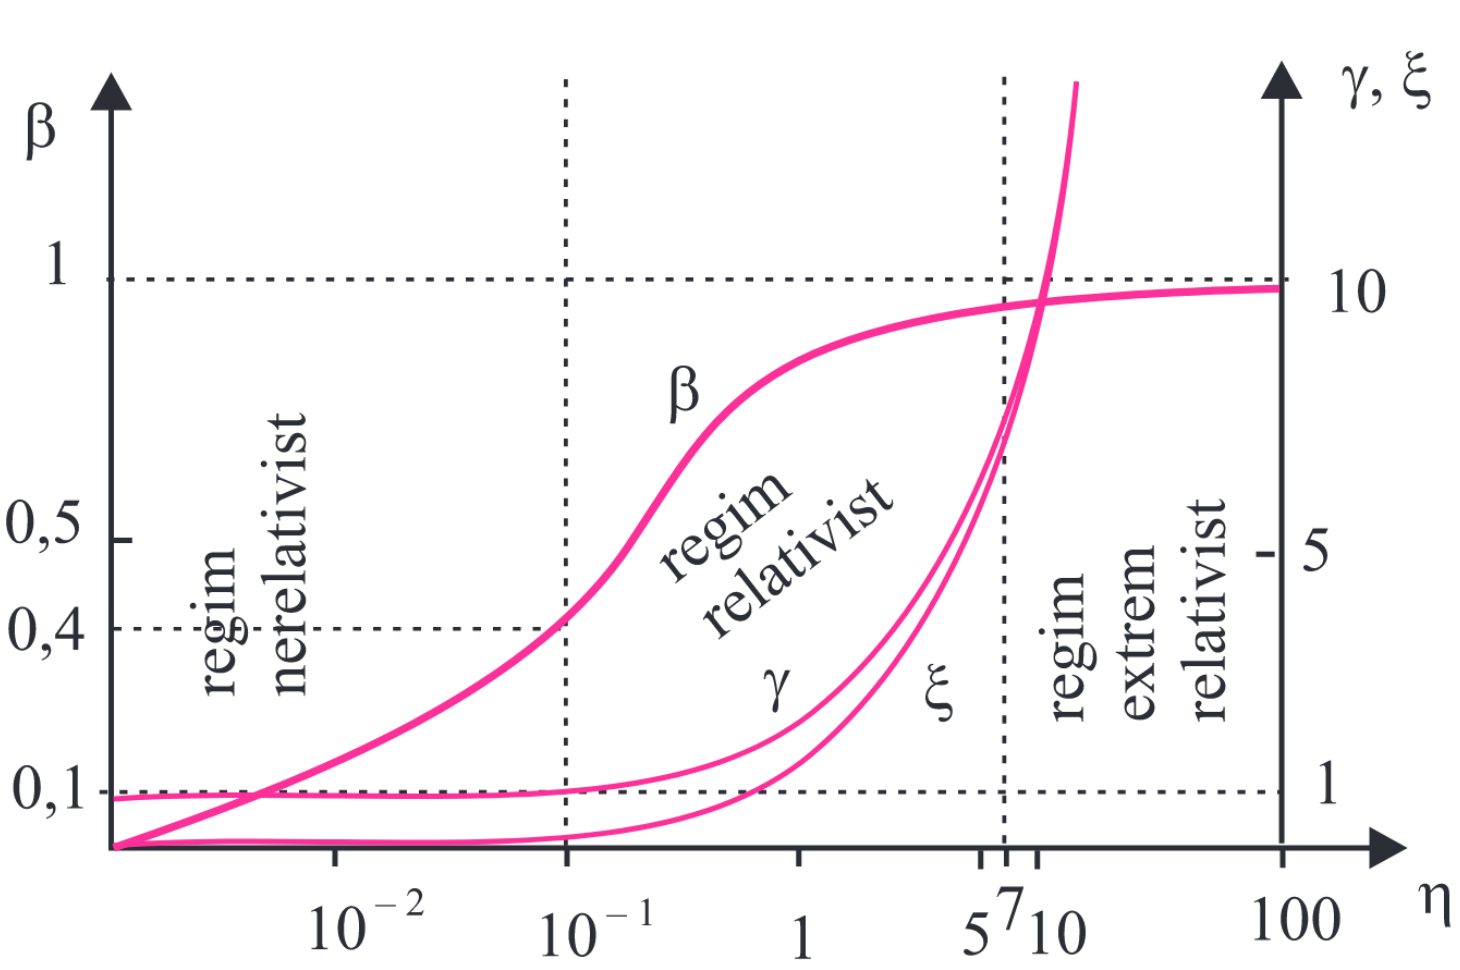
\includegraphics[width=0.45\textwidth]{fig/regimuri}
        \caption{%
            Reprezentare semilogaritmică a dependenței vitezei, energiei, și
            impulsului normate de energia cinetică normată
        }
    \end{wrapfigure}

    În figura 4 este ilustrată variația mărimilor normate $\beta$, $\gamma$,
    și $\xi$ în funcție de energia cinetică normată $\eta$.

    După intervalul cinetic în care iau valori \emph{parametrii reduși}, putem
    delimita trei domenii dinamice:
    \begin{itemize}
        \item domeniul nerelativist, în care masa particulei poate fi considerată
            aproximativ constantă și egală cu masa de repaus
            ($\gamma \approx 1$, $\beta \approx 0,4$).
        \item domeniul relativist, pentru \( 10^{-1} < \eta < 7 \).
        \item domeniul extrem relativist, în care viteza particulei poate fi
            considerată constantă și egală cu viteza luminii ($\beta \approx 1$).
    \end{itemize}
}

În tehnica accelerării particulelor, în fizica atomică și nucleară, se folosesc,
pentru măsurarea energiei și impulsului, unități care nu fac parte din SI, dar
care prezintă avantaje în calculele curente.

Pentru măsurarea energiei unei particule se utilizează de regulă electron-voltul
[eV]. Acesta reprezintă energia câștigată de un electron accelerat sub o
diferență de potențial de 1 V.
\[ 1 ~ \mathrm{eV} = 1,602\cdot10^{-19} ~ \mathrm{J} \]

Deoarece în domeniul extrem relativist impulsul este \( p \approx mc = \frac{E}{c} \),
putem introduce o unitate arbitrară pentru impuls $\left[\frac{eV}{c}\right]$.
\[ 1 \frac{eV}{c} = 5,35\cdot10^{-28} ~ \mathrm{N \cdot s} \]


\clearpage

\section*{Bibliografie}
\begin{itemize}
    \item Manualul de fizică pentru clasa a XII-a \\
        Cleopatra Gherbanovschi, Nicolae Gherbanovschi \\
        Editura NICULESCU ABC \\
        2016
\end{itemize}

\end{document}
